\section{Comparison of Gas Costs}
\label{sec:comparison}

Because all operations are performed within the EVM,
the primary cost metric is the overall gas cost.
Thus, the focus is on minimizing the total gas used.
Ideally, the best algorithm will have the lowest maximum, mean, and median
gas costs.
We note that the results here are different from those
in~\cite{EfficientIsqrt} for three reasons:
first, some of the algorithms are different
(and we chose the most recent version of those found online);
second, we ensure that all input values are unique
(certain values may have been double counted);
third, different input values were chosen.

After analyzing the per-call gas cost distribution,
we discuss the associated costs of deploying the algorithm
to the Ethereum blockchain.


\subsection{Data Point Selection}

Any gas cost comparison requires the selection of \texttt{uint256}
values for input.
The values were chosen in this way:

\begin{itemize}
\item all numbers of the form $2^{k}-1$, $2^{k}$, and $2^{k}+1$
    for positive values of $k$;
\item $v-1$, $v$, and $v+1$ for $v = (2^{128}-1)^{2}$
    (these were chosen because of an edge case in an algorithm);
\item random values chosen according to the
    loguniform distribution~\cite{ScipyLoguniform}
    on $\brackets{1, 2^{256}}$ when the random seed
    is initialized to $0$~\cite{NumpyRandomSeed}.
\end{itemize}

\noindent
The number of random samples were increased until
there were $2048$ unique values.
While it is clear that the particular distribution affects the results,
we believe choosing the input values in this way reduces
the risk of bias.
There were a total of $768$ deterministic values chosen
and a total of $1303$ random samples determined
the remaining 1280 values.

In addition to measuring the gas cost,
the result of each integer square root operation was
validated using
Python's integer square root~\cite{PythonIsqrt,PythonIsqrtLink}.
There was no instance in which an algorithm ever produced an incorrect result;
this is, of course, not a proof that 
\prb{}, \OpenZeppelin{}, and \abdk{} are correct,
but rather that there are no known values where these algorithms fail.


\subsection{Summary Statistics}

\begin{table}[t]
\centering
\begin{tabular}{|c|
    |S[table-format=5.0]|S[table-format=3.0]
    |S[table-format=4.0]|S[table-format=3.0]
    |S[table-format=3.0]|}
\hline
& \Uniswap{} & \prb{} & \OpenZeppelin{} &
    \abdk{} & \python{} \\
\hline
Max    & 34205 & 878 & 1021 & 881 & 963 \\
Mean   & 17734 & 795 &  950 & 803 & 885 \\
Median & 17639 & 798 &  949 & 803 & 888 \\
Std    &  9558 &  34 &   30 &  33 &  44 \\
\hline
\end{tabular}
\caption[Gas Costs Statistics 1]{Here are some statistics
    related to the gas cost data from Figure~\ref{fig:gas_plots_1}.
    We recall that the \Uniswap{} and \python{}
    algorithms are provably correct.
    These results are for the tests in Section~\ref{sec:comparison}.
    }
\label{table:gas_costs_1}
\end{table}

\begin{table}[t]
\centering
\begin{tabular}{|c|
    |S[table-format=3.0]|S[table-format=3.0]
    |S[table-format=3.0]|S[table-format=4.0]
    |S[table-format=4.0]|S[table-format=4.0]|}
\hline
    & \UnrolledOne{} & \UnrolledTwo{} &
    \cellcolor{yellow!25} \UnrolledThree{} &
    \WhileOne{} & \WhileTwo{} & \WhileThree{} \\
\hline
Max    & 858 & 851 & \cellcolor{yellow!25} 831 & 1246 & 1190 & 1177 \\
Mean   & 776 & 775 & \cellcolor{yellow!25} 749 &  853 &  902 &  870 \\
Median & 779 & 777 & \cellcolor{yellow!25} 752 &  898 &  932 &  895 \\
Std    &  42 &  42 & \cellcolor{yellow!25}  41 &  180 &  160 &  141 \\
\hline
\end{tabular}
\caption[Gas Costs Statistics 2]{Here are some statistics
    related to the gas cost data from Figure~\ref{fig:gas_plots_2}.
    We recall that all of these algorithms are provably correct.
    We see that \UnrolledThree{} has the smallest gas costs
    in terms of maximum, mean, and median.
    These results are for the tests in Section~\ref{sec:comparison}.
    }
\label{table:gas_costs_2}
\end{table}

\begin{table}[p]
\centering
\begin{tabular}{|c|
    |S[table-format=6.0]|S[table-format=6.0]
    |S[table-format=6.0]|S[table-format=6.0]
    |S[table-format=6.0]|}
\hline
  & \BitLength{} & \cellcolor{yellow!15} \Linear{} &
    \HyperFour{} & \LookupFour{} & \LookupEight{} \\
\hline
Max      &    833 & \cellcolor{yellow!15}    796 &    826 &    903 &    906 \\
Mean     &    762 & \cellcolor{yellow!15}    739 &    769 &    846 &    849 \\
Median   &    762 & \cellcolor{yellow!15}    739 &    769 &    846 &    849 \\
Std      &     30 & \cellcolor{yellow!15}     28 &     29 &     30 &     30 \\
\hline
Abs Cost & 282605 & \cellcolor{yellow!15} 276105 & 280407 & 301301 & 349214 \\
Rel Cost & 100454 & \cellcolor{yellow!15}  93954 &  98256 & 119150 & 167063 \\
\hline
\end{tabular}
\caption[Gas Costs Statistics 3]{Here are statistics
    related to the gas cost data;
    we also include the absolute deployment gas cost and
    relative deployment gas cost
    (absolute gas cost less 182151 gas,
    the deployment cost of an empty smart contract).
    All of these algorithms are provably correct.
    These results are for the tests in Section~\ref{sec:comparison}.
    }
\label{table:gas_costs_3}
\end{table}


A listing of the summary statistics describing the runs
may be found in Tables~\ref{table:gas_costs_1},
\ref{table:gas_costs_2}, and \ref{table:gas_costs_3}.
From here, we see that the algorithm with the smallest
mean, median, and maximum gas cost is \UnrolledThree{};
the standard deviation of \UnrolledThree{} is minimal as well.
\Linear{} finishes in a close second place.
The fact that \OpenZeppelinTwo{} comes in third is not surprising
given that it is based on \UnrolledThree{}.


\subsection{Detailed Analysis}

We now take a closer look at how the gas cost varies
with the argument.

For each value we tested,
we determined the minimal gas cost
and then counted the number of times each algorithm was minimal;
the results may be found in Table~\ref{table:minimal_gas_costs}.
Additionally, we show a histogram where certain algorithms
were minimal in Figure~\ref{fig:minimal_gas_hist}.
There does not appear to be a particular pattern
in the value distribution.
The main trend is that \UnrolledThree{}
consistently performs well across the range of arguments.
The only region where this does not hold is for small arguments,
where other algorithms (\while{}) performed better;
this makes sense because those values require fewer Newton iterations.

Overall, \UnrolledThree{} has the lowest cost
for a majority of points,
so we declare this to be the algorithm of choice.
A more extensive analysis (with similar results) may be found in
Appendix~\ref{app:extended}.

\begin{table}[p]
\centering
\begin{tabular}{|c|S[table-format=4.0]|}
\hline
Total & 2048 \\
\hline
\Uniswap{}       &    2 \\
\python{}        &    5 \\
\UnrolledOne{}   &    5 \\
\UnrolledTwo{}   &    5 \\
\cellcolor{yellow!25} \UnrolledThree{} & \cellcolor{yellow!25} 1222 \\
\WhileOne{}      &  386 \\
\WhileTwo{}      &  156 \\
\WhileThree{}    &  297 \\
\hline
\end{tabular}
\caption[Minimal Gas Costs Statistics]{Here are number of times
    each method had minimal gas costs;
    methods not included were never minimal.
    These results are for the tests in Section~\ref{sec:comparison}.
    }
\label{table:minimal_gas_costs}
\end{table}

\begin{figure}[p]
\centering
    \begin{subfigure}[t]{0.45\textwidth}
    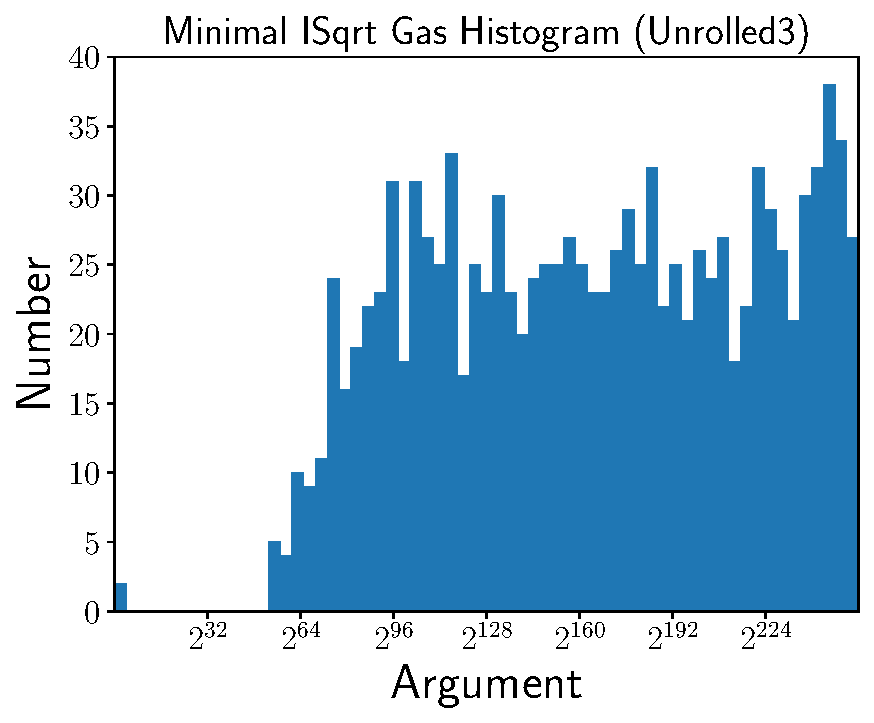
\includegraphics[width=\textwidth]{plots/minimal_hist_Unrolled3.pdf}
    \end{subfigure}
    \begin{subfigure}[t]{0.45\textwidth}
    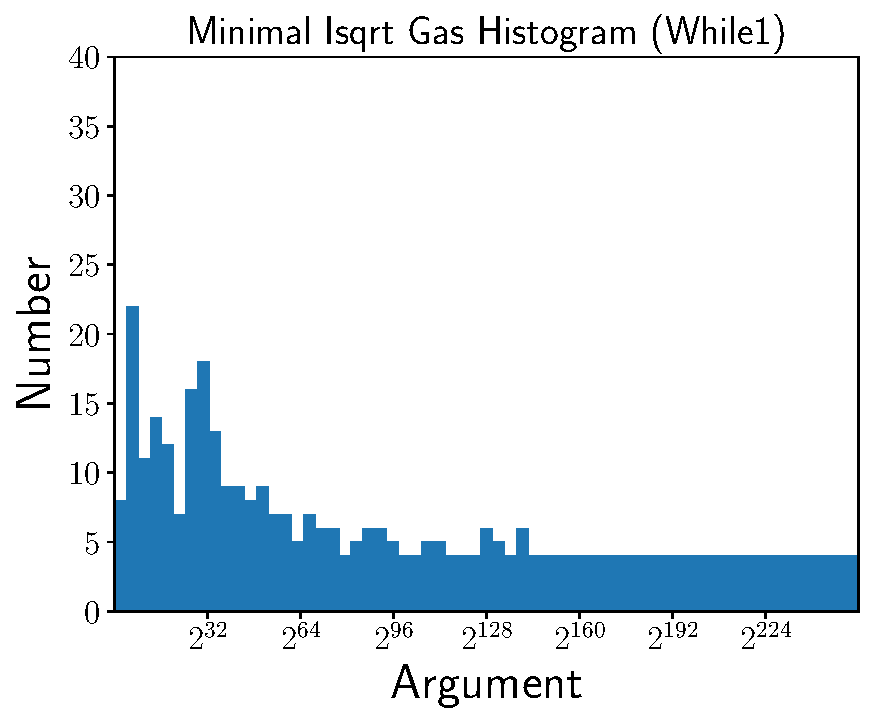
\includegraphics[width=\textwidth]{plots/minimal_hist_While1.pdf}
    \end{subfigure}

    \begin{subfigure}[t]{0.45\textwidth}
    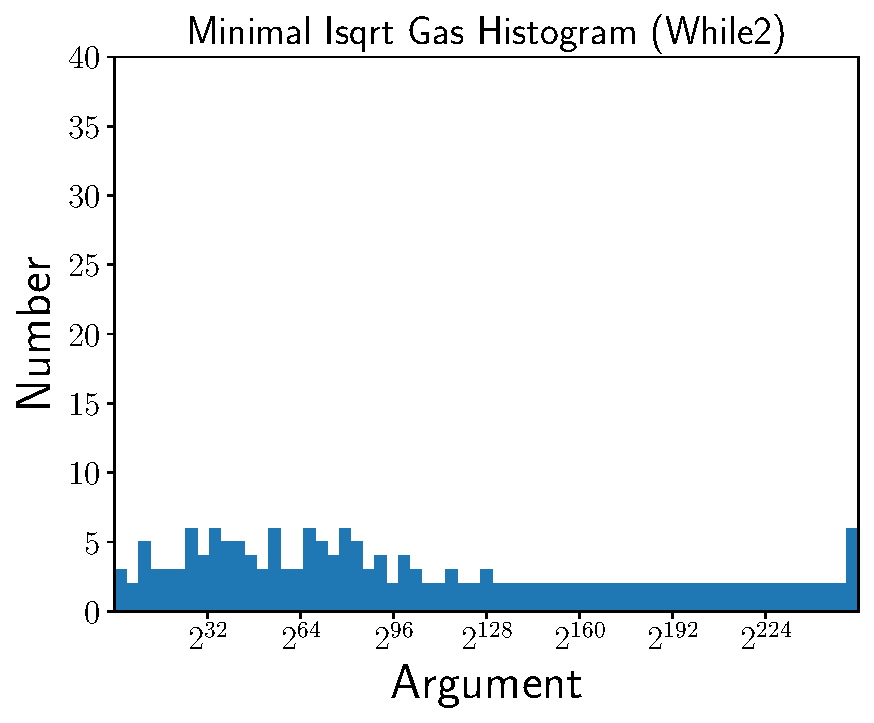
\includegraphics[width=\textwidth]{plots/minimal_hist_While2.pdf}
    \end{subfigure}
    \begin{subfigure}[t]{0.45\textwidth}
    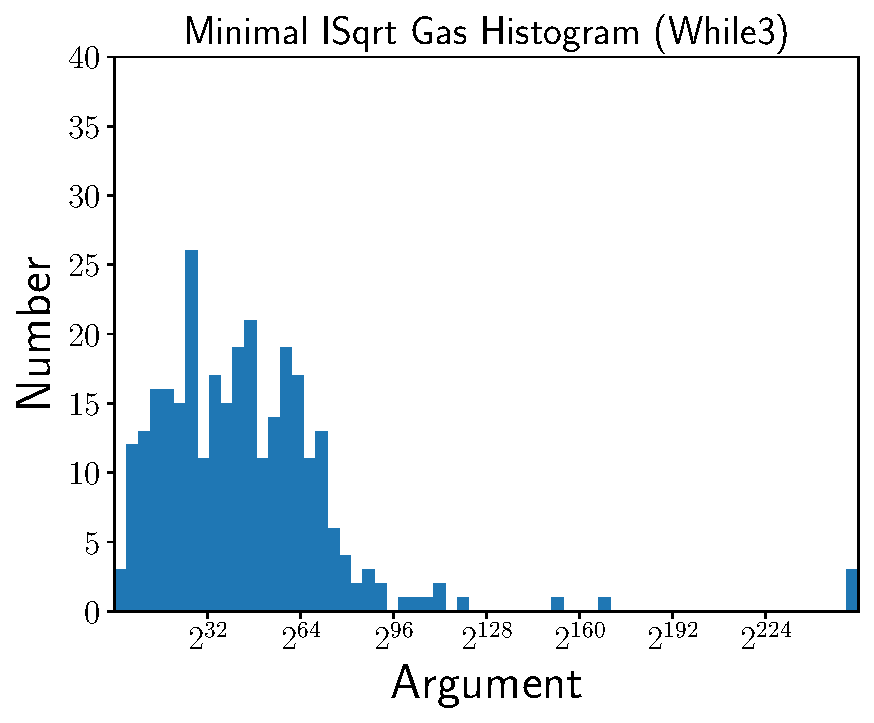
\includegraphics[width=\textwidth]{plots/minimal_hist_While3.pdf}
    \end{subfigure}
    \caption{Here we plot a histogram showing where each algorithm is minimal
        and provides more detail to the results
        in Table~\ref{table:minimal_gas_costs}.
        Each bin counts the total number of instances where the algorithm's
        gas cost is minimal.
        These results are for the tests in Section~\ref{sec:comparison}.
        }
    \label{fig:minimal_gas_hist}
\end{figure}



\subsection{Deployment Gas Cost}

While the primary design criterion is provably-correct algorithm
with efficient operation,
it is important to recognize the initial (one-time) cost
of \emph{deploying} the algorithm to the Ethereum blockchain.

The deployment cost is related to the Ethereum bytecode;
this is the compiled version of the algorithm
which runs on the Ethereum Virtual Machine.
The cost depends on both the size of the bytecode
along with the specific instructions
(different instructions have different gas costs).

In Tables~\ref{table:gas_costs_1}, \ref{table:gas_costs_2},
and \ref{table:gas_costs_3},
we include the absolute and relative deployment costs:
the absolute deployment cost is the gas cost given
by the Hardhat Solidity compiler
(using Solidity version \texttt{0.8.20}
and the optimizer enabled for \texttt{1000000} runs)~\cite{hardhat};
the relative deployment cost is obtained by subtracting
the deployment cost of an empty smart contract
(182151~gas).
We highlight algorithms with relative deployment cost below 95000~gas;
this value was chosen somewhat arbitrarily
but makes it easier to distinguish algorithms
by deployment cost.

Because the cost of deployment is a one-time cost,
the data here is included to provide a larger picture.
The expectation is that minimizing the per-operation cost
is more important than a minimal deployment cost.
Thus, even though \UnrolledThree{} has a slightly larger deployment cost
than \OpenZeppelinTwo{},
it is still thought that \UnrolledThree{} will result
in an overall lower cost.
